
\documentclass[10pt]{beamer}

\usepackage[utf8]{inputenc}
\usepackage[T2A]{fontenc}
\usepackage[russian]{babel}
\usepackage{hyperref}
\usepackage{amsmath}
%\usepackage[footnotes,oglav,spisok,boldsect,eqwhole,kursrab,hyperprint]{project1}
\usetheme{Copenhagen}
\useoutertheme{default}
\usecolortheme{sidebartab}
%\usefonttheme{serif}
\useoutertheme[]{miniframes}
\usepackage{graphicx}
\usepackage{lipsum}
%\usepackage{rumathgrk1}

%\usepackage{glonti}
\defbeamertemplate*{footline}{Warsaw} {%
\leavevmode%
\hbox{%
\begin{beamercolorbox}[wd=.5\paperwidth,ht=2.5ex,dp=1.125ex,leftskip=.3cm,rightskip=.3cm]{author in head/foot}%
\insertframenumber{}%
\hfill\insertshortauthor
\end{beamercolorbox}%
\begin{beamercolorbox}[wd=.5\paperwidth,ht=2.5ex,dp=1.125ex,leftskip=.3cm,rightskip=.3cm]{title in head/foot}%
\usebeamerfont{title in head/foot}\insertshorttitle
\end{beamercolorbox}
}%
\vskip0pt%
}


% \setbeamersize
% {
%     text margin left=0.8cm,
%     text margin right=0.8cm
% }
\renewcommand{\thempfootnote}{\arabic{mpfootnote}}
\title{\textbf{Восстановление человеком исходной позы после толчка \\
Reversion of initial posture by a person after a push}}

\author{\textbf{Романов Андрей Владимирович}}
\institute{\textbf{МГУ им. М.В. Ломоносова}\\\textbf{Механико-математический факультет} 
\\ \textbf{Кафедра прикладной механики и управления}
\\ \textbf{Научный руководитель: Кручинин П.А.}}
\date{\today}



\begin{document}

\maketitle

\begin{frame}{Описание задачи}
	\begin{figure}[h!]
		\begin{center}
			\begin{minipage}[h]{0.33\linewidth}
				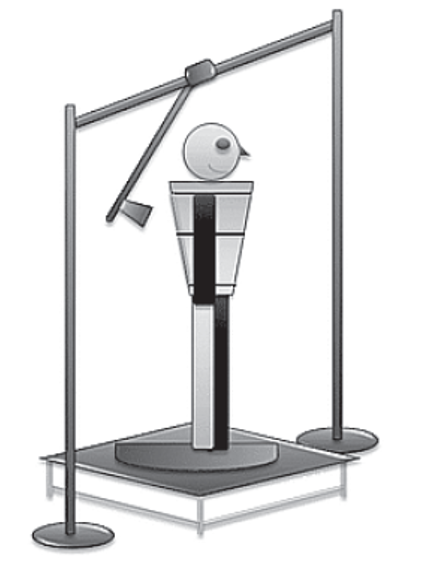
\includegraphics[width=1\linewidth]{images/human.png}
				\caption{Схематическое изображение толкателя
					и положения испытуемого на стабилоплатформе}
			\end{minipage}
			\hfill
			\begin{minipage}[h]{0.66\linewidth}
				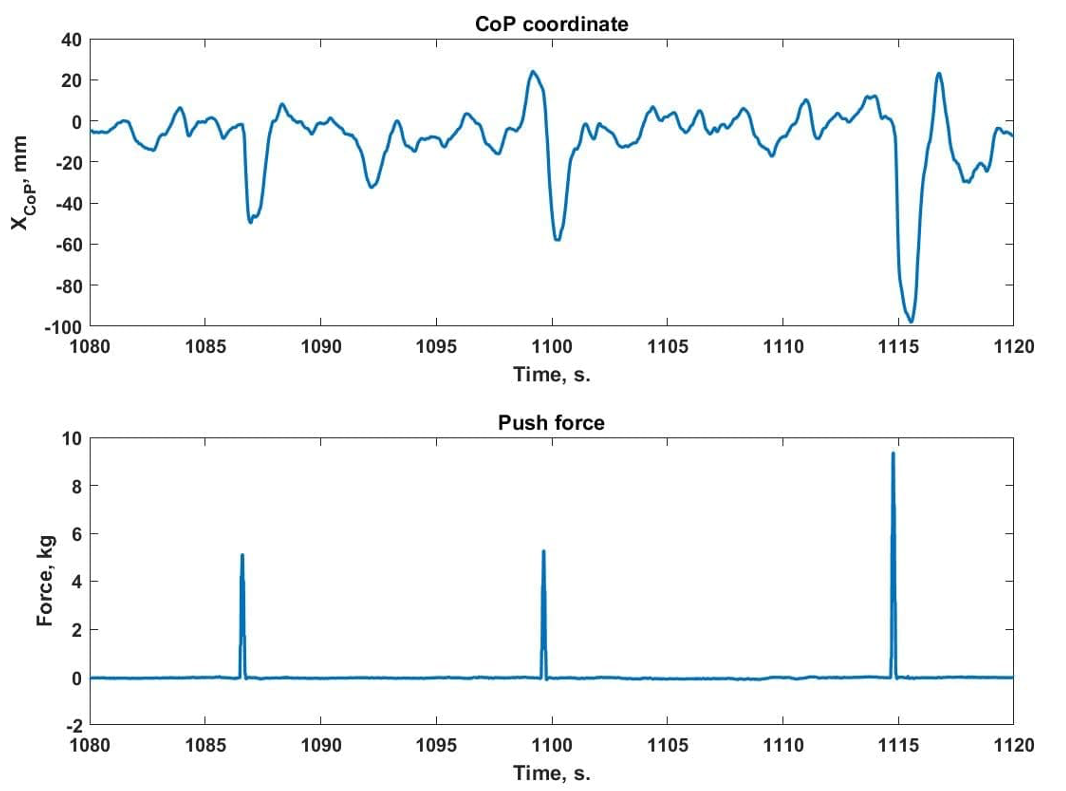
\includegraphics[width=1\linewidth]{images/Pushes.png}
				{\footnotesize
					\caption{Отклонение сагиттальной координаты при различных по силе толчках (данные предоставлены сотрудниками ИМБП РАН) }
				}
			\end{minipage}
		\end{center}
	\end{figure}
\end{frame}

\begin{frame}{Задача быстродействия}
	\begin{columns}
		\column{0.55\textwidth}
		\begin{figure}[h!]
			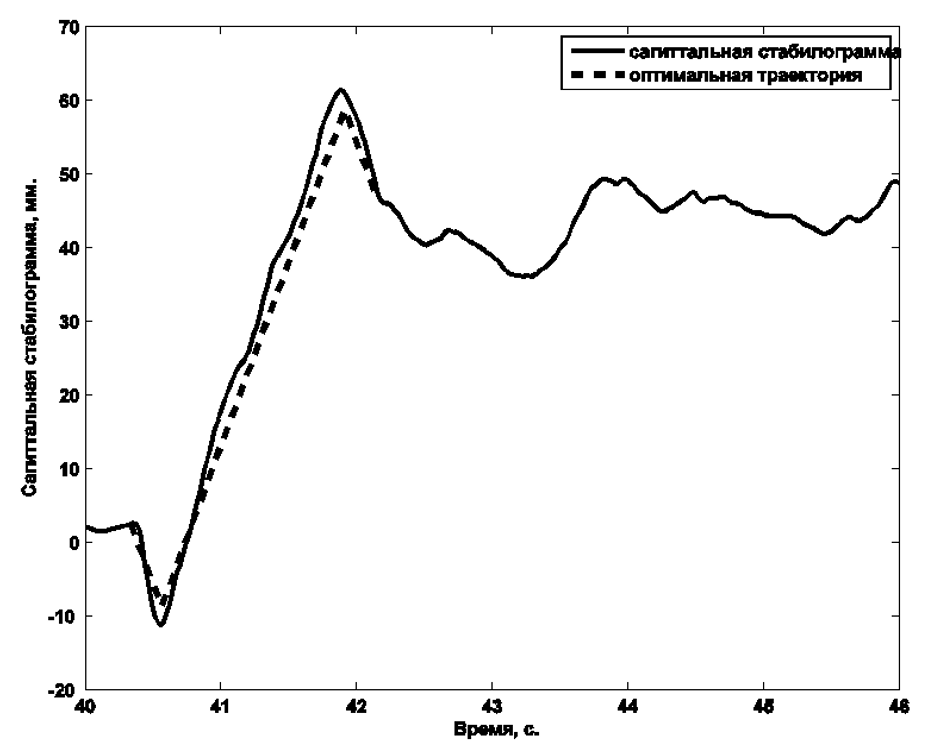
\includegraphics[width=1\linewidth]{images/stabilos.png}
			\caption{Характерный вид сагиттальной стабилограммы при наклоне при выполнении теста со ступенчатым
			 воздействием}
		\end{figure}
		\column{0.6\textwidth}
		% \column{\dimexpr\paperwidth-2pt}
		В работе рассматриваются возможные алгоритмы управления изменением
		позы человека, основанные на решении задачи оптимального быстродействия,
		которые можно было бы использовать для возвращения человека в исходную 
		вертикальную позу. В качестве математической модели используется модель
		«перевернутого маятника». Это решение предлагается использовать для
		оценки эффективности управления человеком при возвращении в
		вертикальную позу, путем сравнения времени реального процесса с полученным
		эталонным решением оптимальной задачи.
	\end{columns}
\end{frame}

\begin{frame}{Математическая модель}
	Рассматривается задача возвращения в исходную позу после завершения толчка
	\begin{columns}
		\column{0.62\textwidth}
		\begin{figure}[h!]
			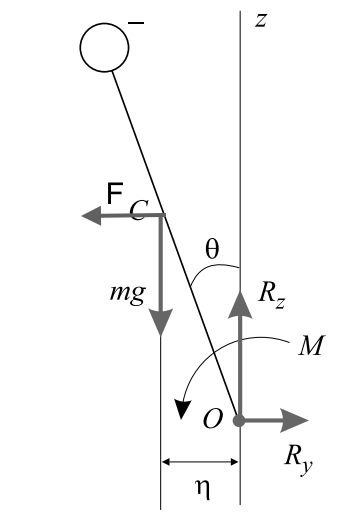
\includegraphics[width=0.6\linewidth]{images/body_1.png}
			\caption{Модель перевернутого маятника}
		\end{figure}
		\column{0.5\textwidth}

		\[
			J\ddot{\varphi}=m_Tgl\varphi+M
		\]
		\[
			\varphi(0)=\varphi_0,\, \dot{\varphi}(0)=\omega_0
		\]
		\[
			\varphi(t)=\varphi_k,\, \dot{\varphi}(t_k)=0
		\]
		\[
			M(0)=M(t_k)=-m_Tgl\varphi_k
		\]
		\[
			U^-\leq\dot{M}\leq U^+
		\]
	\end{columns}
\end{frame}
\begin{frame}{Решение задачи быстродействия}
	В прошлом году решалась задача быстродействия

	Система разбивается на 3 этапа, с чередованием знака управления

	Решение сводится к отысканию корней полинома для нахождения времени возвращения в вертикальную позицию.

	$\theta - \text{угол отклонения от вертикали}$

	$\omega - \text{угловая скорость тела}$

	$m - \text{момент, возникающий в голеностопном суставе}$


	\begin{columns}
		\column{0.5\textwidth}
		\begin{equation}\label{basesystem}
			\left\{ {\begin{aligned}
						 & \theta^{'} = \omega , \hfill   \\
						 & \omega^{'} = \theta+m , \hfill \\
						 & m^{'} = u . \hfill             \\
					\end{aligned}} \right.
		\end{equation}
		\column{0.5\textwidth}
		\[
			u=
			\begin{cases}
				-u_{max} \\
				+u_{max}
			\end{cases}
		\]\\*
	\end{columns}
	
\[
    \tau=\frac{t}{t_\ast},\ t_\ast=\sqrt{\frac{J}{m_Tgl}},\ \varphi_\ast=\varphi_0-\varphi_k
\]
	\[
		\theta(0)=1;\ \theta^{'}(0)=\frac{t_\ast}{\varphi_\ast}\omega_0=\Omega_0;\ m(0)=0
	\]
	\[
		\theta(\tau_f)=0;\ \theta^{'}(\tau_f)=0;\ m(\tau_f)=0
	\]
\end{frame}
\begin{frame}{Решение задачи быстродействия}
	Запишем функцию Понтрягина
\[
    H(\psi(t),y(t),u(t))=\psi_1\cdot\omega+\psi_2\cdot(\theta+m)+\psi_3\cdot u
\]

\begin{equation} \label{7}
    \left\{ {\begin{aligned}
                 & \psi^{'}_1=  - \frac{{\partial H}}{{\partial \theta}} = - \psi_2\hfill  \\
                 & \psi^{'}_2=  - \frac{{\partial H}}{{\partial \omega }} = - \psi_1\hfill \\
                 & \psi^{'}_3=  - \frac{{\partial H}}{{\partial m }} = - \psi_2 \hfill     \\
            \end{aligned}} \right.
\end{equation}
При $\psi_3\equiv0$ следует, что $\psi_2\equiv0$ и $\psi_1\equiv0$ следовательно особого управления нет.

Тогда для условия максимизации функции Понтрягина
\[
    u=
    \begin{cases}
        -u_{max}, & \text{при $\psi_3<0$}          \\
        +u_{max}, & \text{при $\psi_3\geqslant 0$}
    \end{cases}
\]\\*
\end{frame}
\begin{frame}{Решение задачи быстродействия}
Решая систему \eqref{7}, получим
\[
    \left\{ {\begin{aligned}
                 & \psi_1 = -C_1e^\tau+C_2e^{-\tau}+C_3, \hfill  \\
                 & \psi_2 = C_1e^\tau+C_2e^{-\tau} , \hfill      \\
                 & \psi_3 = -C_1e^\tau+C_2e^{-\tau}+C_3 . \hfill \\
            \end{aligned}} \right.
\]
Анализируя корни уравнения $\psi_3(\tau)=0$, для различной комбинации
коэффициентов $C_1,C_2,C_3$, получим, что число корней не может быть больше двух. В системе может быть не более двух переключений $u$.

Пусть первое переключение управления происходит в момент времени
$\tau=\tau_1$, а второе в момент времени
$\tau=\tau_2$. Рассмотрим систему \eqref{basesystem} на трех этапах,
при переходе между которыми меняется управление.


\end{frame}


\begin{frame}{Решение задачи быстродействия}
	Этап 1. $u=-u_*$ начальные условия
\[
    m(0)=0;\ \theta(0)=1;\ \omega(0)=\Omega_0;
\]

\[
    \left\{ {\begin{aligned}
                 & 0 = -\tau  u_*+c_1, \hfill                                                            \\
                 & 1 = \frac{1}{2} e^{-\tau } \left(C_1 \left(e^{\tau }-1\right)^2+C_2 \left(e^{2
                \tau }+1\right)+C_3 e^{2 \tau }-C_3+2 e^{\tau } \tau  u_*\right) , \hfill                \\
                 & \Omega_0 = \frac{1}{2} e^{-\tau } \left(C_1 \left(e^{2 \tau }-1\right)+C_2 \left(e^{2
                \tau }-1\right)+C_3 e^{2 \tau }+C_3+2 e^{\tau } u_*\right)  . \hfill                     \\
            \end{aligned}} \right.
\]

\[
    \left\{ {\begin{aligned}
                 & m_1(\tau) = -\tau  u_*, \hfill                                                                         \\
                 & \theta_1(\tau) = \frac{e^\tau+e^{-\tau}}{2}+\frac{\Omega_0-u_*}{2}(e^\tau-e^{-\tau})+\tau u_* , \hfill \\
                 & \omega_1(\tau) =\frac{e^\tau-e^{-\tau}}{2}+\frac{\Omega_0-u_*}{2}(e^\tau+e^{-\tau})+u_*   . \hfill     \\
            \end{aligned}} \right.
\]
Аналогично для 2 и 3 этапов
\end{frame}
\begin{frame}{Решение задачи быстродействия}
	Условие сопряжения этих интервалов
\[
    \left\{ {\begin{aligned}
                 & m_2(\tau_2) = m_3(\tau_2), \hfill            \\
                 & \theta_2(\tau_2) =  \theta_3(\tau_2), \hfill \\
                 & \omega_2(\tau_2) = \omega_3(\tau_2) . \hfill \\
            \end{aligned}} \right.
\]
	Замена переменных
\[
    x=e^{\tau_1} ,\,\,y=e^{\tau_2} ,\,\,z=e^{\frac{\tau_f}{2}}
\]
		\begin{figure}[h!]
			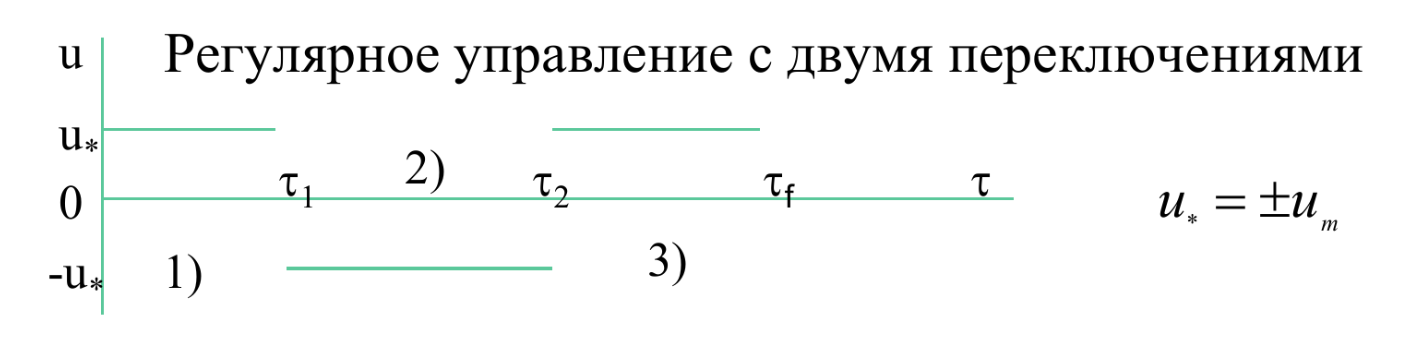
\includegraphics[width=0.8\linewidth]{images/control_intervals.png}
			\caption{Интервалы переключения управления}
		\end{figure}

\end{frame}
	
\begin{frame}{Решение задачи быстродействия}
	Требуется отобрать наименьший корень уравнений больший 1. При различных по знаку $u_*$.
	
		\begin{columns}
			\column{1\textwidth}
			\begin{equation}\label{koshisystem}
				 {\begin{aligned}
					& x=\left( \frac{1}{2z}-\frac{u_*z}{2}-(\Omega_0-u_*)\frac{1}{2z}\right)\frac{z}{u_*(1-z)} \hfill	\\
					& y=zx, \hfill                                                                                              \\
			   \end{aligned}}
			\end{equation}
			\begin{equation}\label{koshisystem}
				\left[ {\begin{aligned}
					& u_*z^2+\Omega _0-1-u_*=0, \hfill    \\
					& (-u_* \Omega _0+u_*^2-u_*)z^4-4 u_*^2z^3+(2 u_* \Omega _0+6 u_*^2-\Omega _0^2+1)z^2- \hfill \\
					& -4 u_*^2z+-u_* \Omega _0+u_*^2+u_*=0                                                                                           \\
			   \end{aligned}} \right.
			\end{equation}
		\end{columns}
		$\tau_f=\ln(z)$

\end{frame}

\begin{frame}{Определение начальных условий для задачи быстродействия}
	Для корректного решения задачи быстродействия необходимо определить начальные условия после толчка.
	
	\hfill \\
	Для этого необходимо построить оценку $\tilde{\eta}$ траектории центра масс системы, зная траекторию центра давления,
	и взять значение $\tilde{\eta_0}$ и $\tilde{\dot{\eta_0}}$ в момент времени завершения толчка

\end{frame}

\begin{frame}{Связь центра масс и центра давления}
		\begin{columns}
		\column{0.5\textwidth}
		\begin{figure}[h!]
			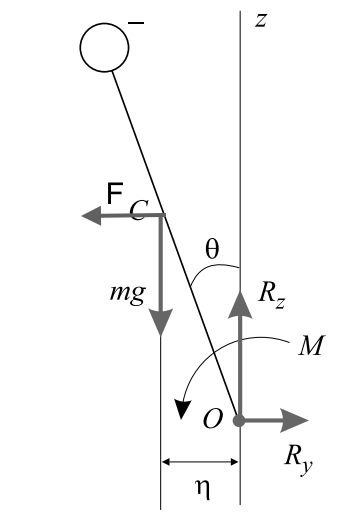
\includegraphics[width=0.7\linewidth]{images/body_1.png}
			\caption{Силы действующие на модель стержня, имитирующего тело человека}
		\end{figure}
		\column{0.5\textwidth}
		\begin{figure}[h!]
			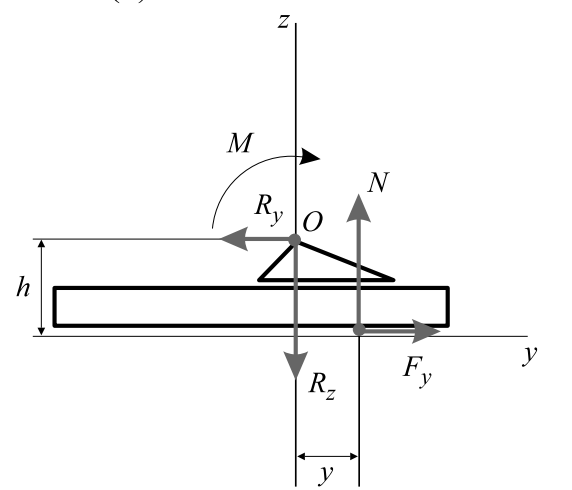
\includegraphics[width=0.8\linewidth]{images/foot.png}
			\caption{Силы действующие на на систему «стопы ног – платформа стабилоанализатора» }
		\end{figure}
	\end{columns}

\end{frame}

\begin{frame}{Связь центра масс и центра давления}
	\begin{columns}
	\column{0.5\textwidth}
	\begin{equation}\label{koshisystem}
    \left\{ {\begin{aligned}
                 & ml\ddot{\theta} = -R_y-F , \hfill   \\
                 & 0=R_z-mg, \hfill \\
                 & J \ddot{\theta} = mlg\theta-Fl_1+M_x . \hfill             \\
            \end{aligned}} \right.
\end{equation}
	\column{0.5\textwidth}
	\begin{equation}\label{koshisystem}
		\left\{ {\begin{aligned}
					 & M_x = Ny+F_yh , \hfill   \\
					 & F_y = R_y , \hfill \\
					 & N \approx mg . \hfill             \\
				\end{aligned}} \right.
	\end{equation}
\end{columns}

	$$M_x=mgy-h\left(F+ml\ddot{\theta}\right)$$

	$$\left(J+mlh\right)\ddot{\theta}=mgl\theta+mgy-Fl_1-Fh$$ 


 	$$\frac{(J+mlh)l\ddot{\theta}}{mgl}=l\theta+y-\frac{F}{mg}(l_1+h);\quad \text{Замена: }\eta=-l\theta; \quad T^2=\frac{J+mlh}{mgl};$$
\begin{equation}\label{eta_y}
	T^2\ddot{\eta}=\eta-y+\frac{F}{mg}(l_1+h)
\end{equation}

\end{frame}

\begin{frame}{Связь центра масс и центра давления}
	Cоотношение \eqref{eta_y} предлагается использовать для определения начальных условий движения сразу после толчка
	
	\hfill \\
	Далее необходимо построить оценку $\tilde\eta$ движения центра масс различными способами, описанными в работах, выполненых под руководством П.А. Кручинина
\end{frame}

\begin{frame}{Моделирование движения человека}
	Модель движения человека, где $M=-C\theta-P\dot\theta$ - момент в голеностопе
		$$J\ddot{\theta}=mgl\theta+M-Fl_1$$
	\begin{columns}
		\column{0.5\textwidth}
		\begin{figure}[h!]
			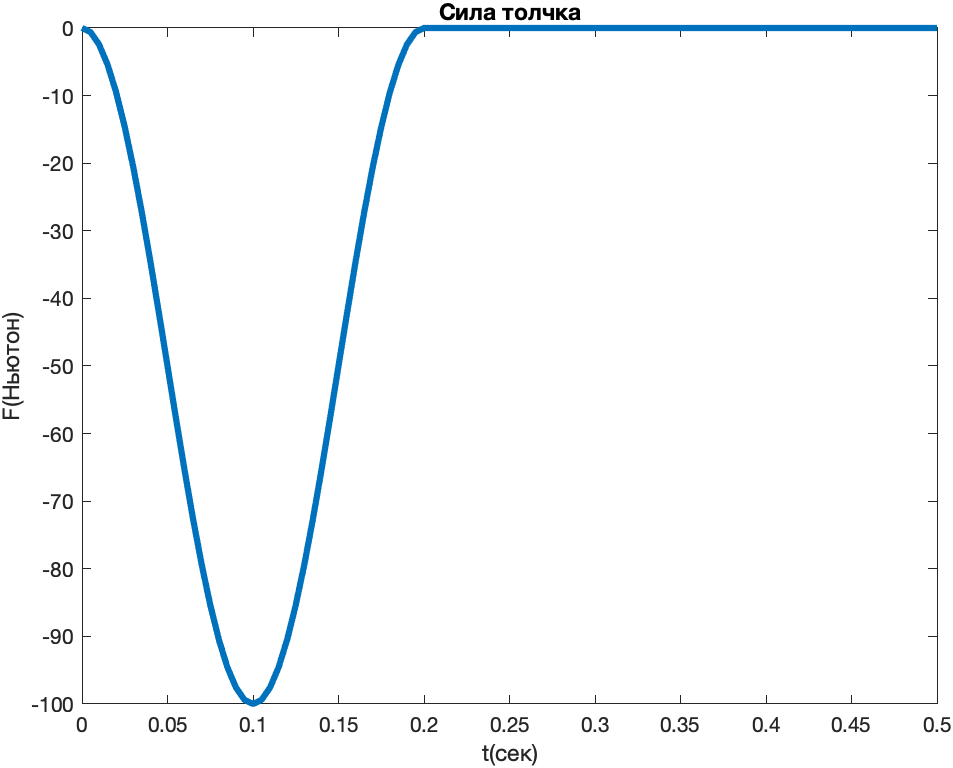
\includegraphics[width=1\linewidth]{images/pushes_my_1.png}
			\caption{Модель силы толчка}
		\end{figure}
		\column{0.5\textwidth}
		\begin{figure}[h!]
			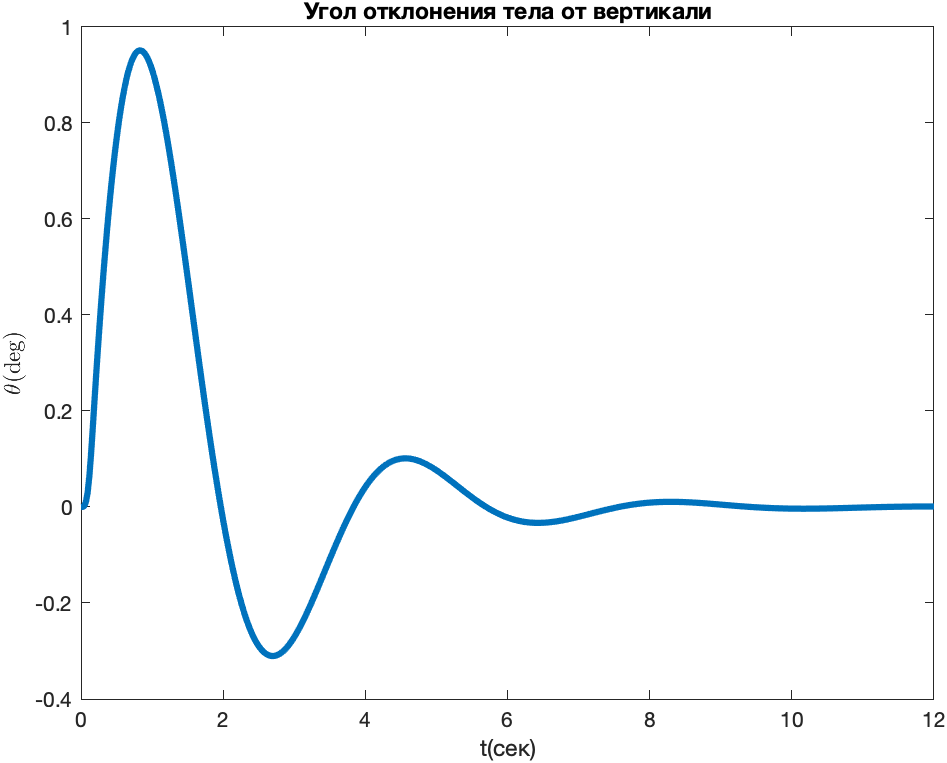
\includegraphics[width=1\linewidth]{images/deg_my_1.png}
			\caption{Модель изменения угла отклонения}
		\end{figure}
	\end{columns}
\end{frame}

\begin{frame}{Алгоритм фильтрации (композиция двух фильтров)}

Передаточная функция системы (\ref*{eta_y}) имеет вид 
\[
	G(s)=-\frac{1}{T^2s^2-1}
\]
Ее можно представить в виде композиции двух фильтров
\[
	G(s)=G_1(s)\cdot G_2(s) 
\]
\[
	G_1(s)=\frac{1}{Ts-1}, G_2(s)=\frac{1}{Ts+1}
\]
Оценка координаты центра масс может быть найдена, путем последовательного применения двух фильтров
\[
	T \dot{x}+x=-y \text{ в прямом времени}
\]
\[
	T \dot{\eta}-\eta=x \text{ в обратном времени}
\]

\end{frame}

\begin{frame}{Алгоритм фильтрации (преобразование Фурье)}
	$Y(\omega),N(\omega) - \text{Фурье образы y(t) и $\eta$(t)}$
	\[
		N(\omega)=G(i\omega)\cdot Y(\omega)
	\]
	Представим $y(t)=a(t-t_0)+b+\delta(t)$ 

	$a=\frac{y(t_f)-y(t_0)}{t_f-t_0}, b=y(t_0)$, тогда оценка координаты центра масс может быть найдена из

	$\eta(t)=a(t-t_0)+b+\chi(t)$, где $\chi(t)$ - Фурье праобраз $N(\omega)$
	
\end{frame}

\begin{frame}{Моделирование движения человека}
	\begin{figure}[h!]
		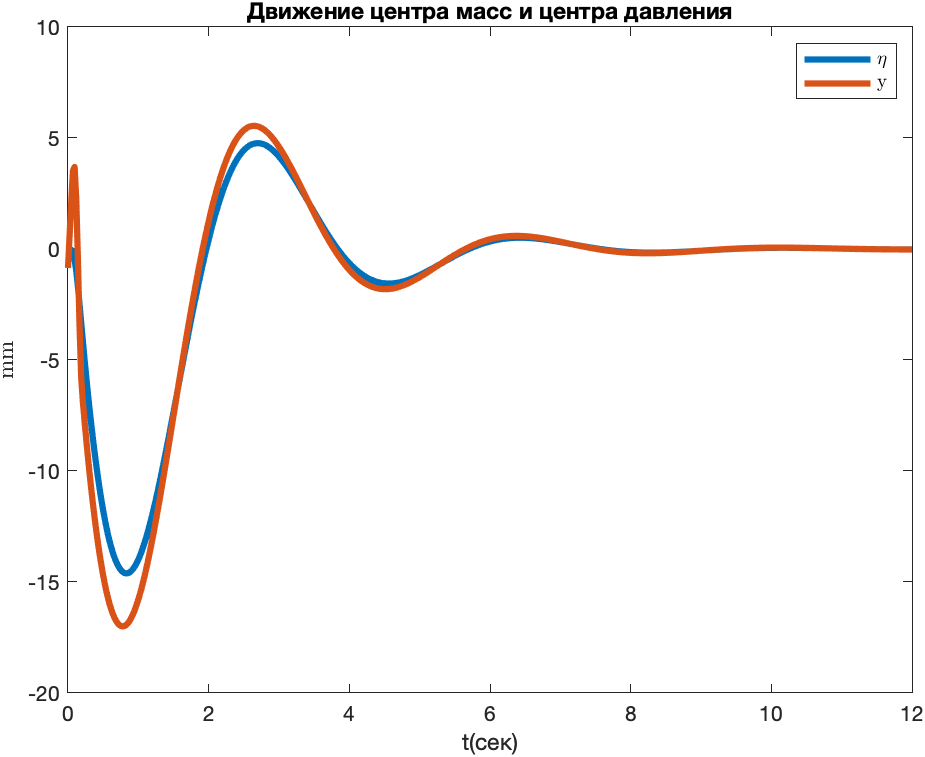
\includegraphics[width=0.7\linewidth]{images/cm_my_1.png}
		\caption{Модель изменения саггитальной координаты центра масс и центра давления}
	\end{figure}
\end{frame}
\begin{frame}{Модельная оценка центра масс с использованием FFT}
	\begin{columns}
		\column{0.5\textwidth}
		\begin{figure}[h!]
			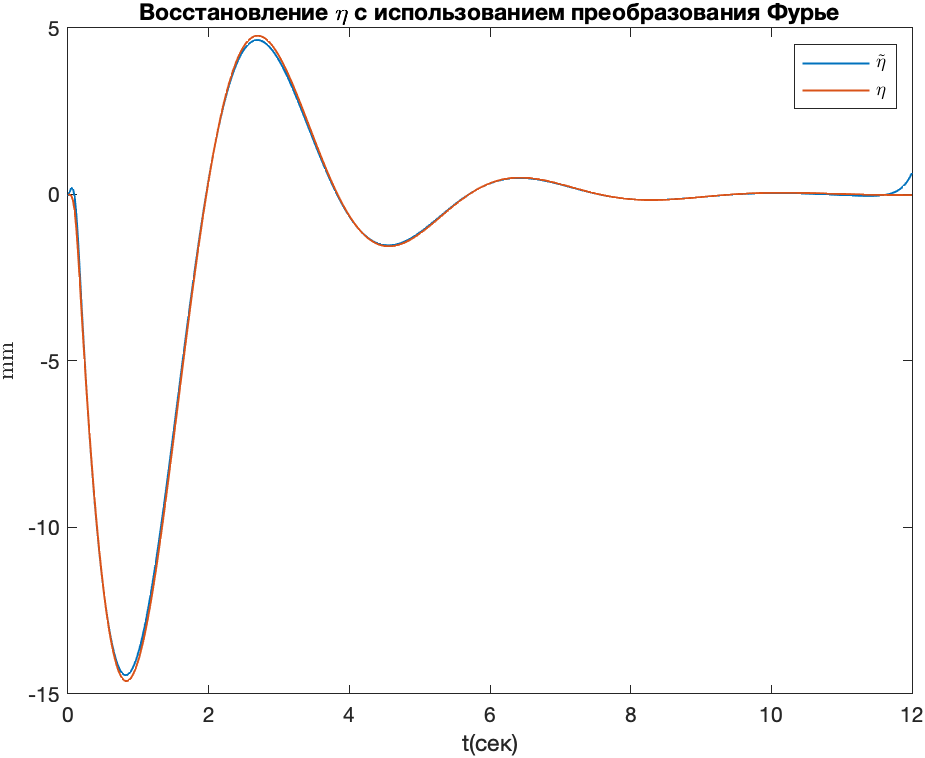
\includegraphics[width=1\linewidth]{images/eta_after_FFT.png}
			\caption{Реальное и восстановленное значение $\eta$}
		\end{figure}
		\column{0.5\textwidth}
		\begin{figure}[h!]
			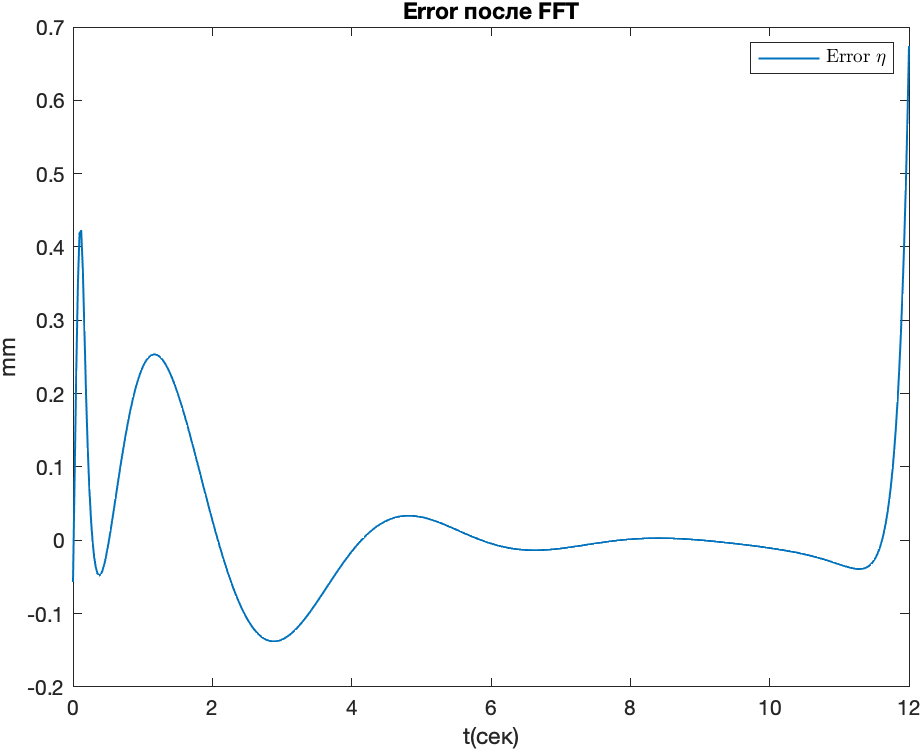
\includegraphics[width=1\linewidth]{images/error_after_fft.png}
			\caption{Ошибка оценивания}
		\end{figure}
	\end{columns}
	$\sigma=0.1mm$
\end{frame}
\begin{frame}{Модельная оценка центра масс с использованием двойной фильтрации}
	\begin{columns}
		\column{0.5\textwidth}
		\begin{figure}[h!]
			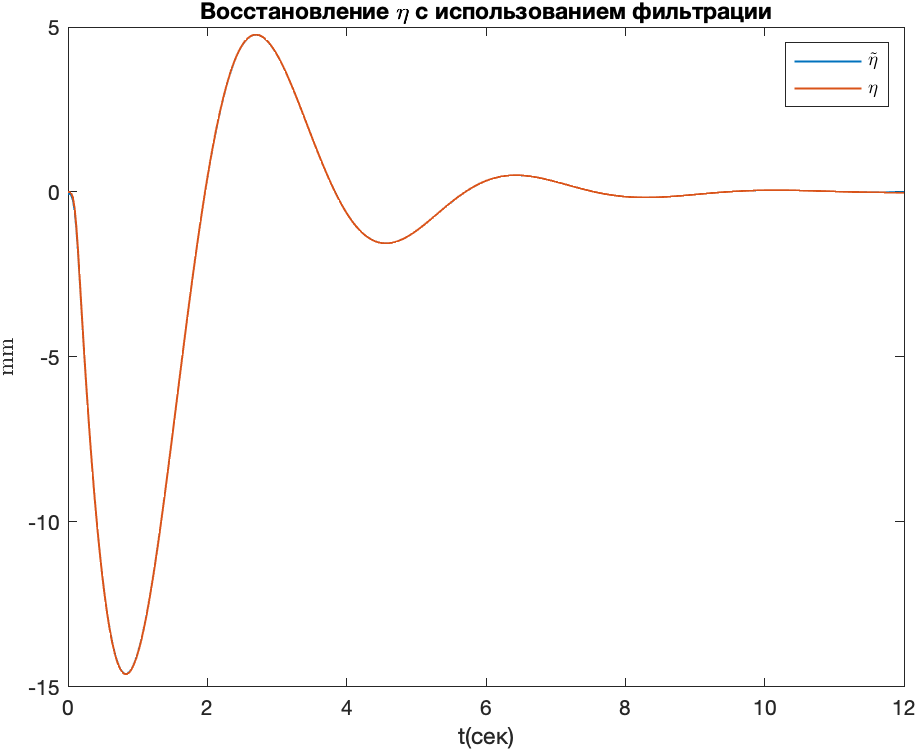
\includegraphics[width=1\linewidth]{images/eta_after_filtering.png}
			\caption{Реальное и восстановленное значение $\eta$}
		\end{figure}
		\column{0.5\textwidth}
		\begin{figure}[h!]
			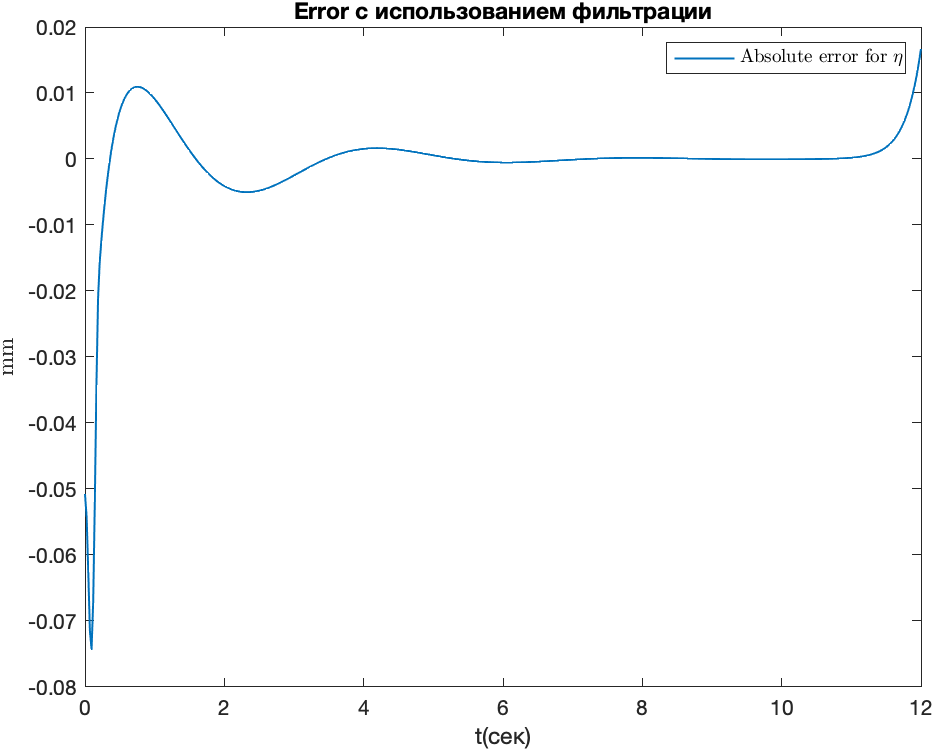
\includegraphics[width=1\linewidth]{images/error_efter_filtering.png}
			\caption{Ошибка оценивания}
		\end{figure}
	\end{columns}
$\sigma=0.008mm$
\end{frame}
\begin{frame}{Дальнейшие шаги}
	\begin{enumerate}
		\item Применить алгоритм двойной фильтрации и фильтрации через FFT для реальных показаний со стабилоанализатора
		\item Получить оценку ц.м. и оценку скорости изменения ц.м. в момент времени завершения толчка
		\item Определить характерную среднюю скорость изменения момента в голеностопе на участках возврата и подставить ее в управление $u_{\ast}=\frac{\dot{M}_{max}}{mgl\varphi_\ast t_\ast}$
		\item Сравнить реальное время возвращения в вертикальную позу с полученными при решении задачи быстродействия
		\item Построить траекторию центра масс при управленнии, полученном при решении задачи быстродействия
	  \end{enumerate}
	
\end{frame}
\begin{frame}{Список основной используемой литературы}

\begin{thebibliography}{15}
	\bibitem{PAKrychinin}П.А. Кручинин Анализ результатов стабилометрических тестов со ступенчатым воздействием с точки зрения механики управляемых систем
    // Биофизика. – 2019. – Т. 64, №5. – С. 1–11.
	\bibitem{mechmodel}П.А. Кручинин Механические модели в стабилометрии // Российский журнал биомеханики. – 2014. – Т. 18, №2. – С. 184–193.
	\bibitem{podoprihin}П.А. Кручинин, М.А. Подоприхин, И.Д. Бекеров Сравнительный анализ алгоритмов оценки движения центра масс по результатам стабилометрических измерений // Биофизика – 2021. – Т. 66, №5. – С. 997–1004. 
	\bibitem{Optimal} Александров В.В., Лемак С.С., Парусников Н.А. Лекции по механике управляемых систем. Москва, Механико-математический факультет МГУ, 2020, 165 с.
	\bibitem{atansfalb}Фалб Питер Л., Атанс Майкл Оптимальное управление, Машиностроение, 1968, 764 с.
\end{thebibliography}
\end{frame}
\end{document}